\section{PDE Discretization}
Multidimensional topological optimization problems often involve the use of partial differential equations (PDEs) which model the physical properties of the materials involved. Most of these PDEs cannot be uniquely solved analytically, so we turn to numerical methods in order to approximate their solutions. The first step in many of these methods is to discretize our domain; that is, we want to choose some scheme to divide our continuous domain into a finite number of pieces over which we will apply a particular method to approximate solutions to the PDE.

In the SIMP method, the Finite Volume Method is used to discretize and approximate solutions to the heat equation for our heat generating medium. We will introduce the Heat Equation and then proceed to give an overview of the Finite Volume Method.
\subsection{The Heat Equation}
Consider a stationary object of that has heat flowing between its interior regions. The temperature at any point in the interior of the object will depend on the spatial position chosen as well as the time we measure the temperature at that point. Therefore, the temperature ($T$) at any point in such an object is a function of both space ($\vec{x}$) and time ($t$) coordinates: $T(\vec{x},t)$.
Physical principles demand that such a temperature function must satisfy the equation
\begin{equation}
	\frac{\partial T}{\partial t}=\nabla\cdot\left(k(\vec{x})\nabla T\right)\label{eqn:HeatEq},
\end{equation}
where $\nabla$ is the gradient operator and the function $k$ represents the thermal diffusivity at a point in our object.

Equation \eqref{eqn:HeatEq} is commonly referred to as the Heat or Diffusion Equation. If we were to have a constant thermal diffusivity throughout our object, it would be possible to analytically find a solution to this partial differential equation. However, as in the problems of interest throughout this paper, when $k$ is not constant we must turn to numerical methods to find approximate solutions for the function $T$.

\begin{figure}
	\centering
	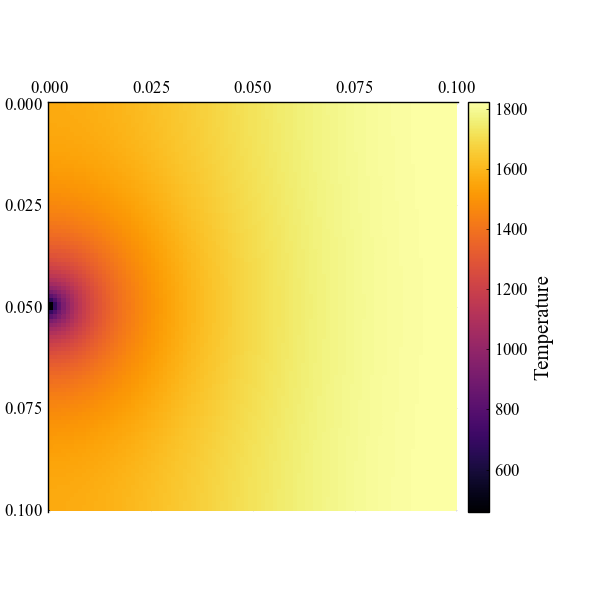
\includegraphics[width=0.8\textwidth]{Chapter_I_Background/Images/Heatmap_Example.png}
	\caption[Heatmap Example]{Heatmap for a \SI{0.1}{\meter} $\times$ \SI{0.1}{\meter} object with uniform heat generation and a heat sink at the center of its west boundary. This map was produced via the Finite Volume Method using $100\times 100$ uniform control volumes.}
\end{figure}

\subsection{The Finite Volume Method}

For our numerical approximations of PDEs in this paper we used the Finite Volume Method (FVM), which will be described in this section.

As with any other numerical method to solve PDEs, we must first discretize our domain by creating some sort of mesh. One major advantage of the Finite Volume Method is that we have a great amount of freedom in choosing our mesh. In FVM the domain can be discretized into a mesh of arbitrary polygons, but we chose uniform squares in our work to simplify the resulting calculations.

Given a mesh of polygons on our domain $\Omega$ with vertices at $\lbrace x_i\rbrace\subset\Omega$, we create a set of {\color{baystate}\textit{control volumes}} around each $x_i$. The resulting set of control volumes discretize the partial differential equation. The Finite Volume Method has us integrate our PDE over each control volume and then use the {\color{tiananmen}Divergence Theorem} to convert these volume integrals into surface integrals involving the fluxes across the boundaries of the control volumes. We then approximate those fluxes across the boundaries to calculate approximate solutions to our PDE.

\begin{thm}[The Divergence Theorem]
	Suppose that $\mathcal{V}$ is a compact subset of $\mathbb{R}^n$ that has a piecewise smooth and positively oriented boundary $\mathcal{S}$ (i.e. $\partial\mathcal{V}=\mathcal{S}$). If $\mathbf{F}$ is a continously differentiable vector field defined on a neighborhood of $\mathcal{V}$, then
	\begin{equation}
		\iiint\limits_{\mathcal{V}}\left(\nabla\cdot\mathbf{F}\right)\dif\mathcal{V}=\oiint\limits_{\mathcal{S}}\mathbf{F}\cdot\dif\mathcal{S}.\label{eqn:div-thm}
	\end{equation}
	\label{thm:div-thm}
\end{thm}

The divergence theorem is the key component in the finite volume method because it allows us to look at fluxes across the boundaries of each control volume, rather than the control volume itself.

Let's look at the finite volume method applied to the heat equation in two dimensions. Suppose we have discretized our space by dividing it up into a mesh of control volumes $\lbrace V_i\rbrace$. We integrate the heat equation PDE over each control volume, using the divergence theorem to convert the volume integral into a surface integral:

$$\int_{V_i}\frac{\partial T}{\partial t}\dif\vec{x}=\int_{V_i}\nabla\cdot \left(k(\vec{x})\nabla T\right)\dif\vec{x}\underset{\eqref{eqn:div-thm}}{=}\int_{\partial V_i}k(\vec{x})\nabla T\cdot\dif s,$$

where $s$ represents the lines that form the boundary of the control volume. Then, applying an approximation scheme to this result, we obtain a sparse and structured linear system.

One other major advantage of the finite volume method is that boundary conditions can easily be taken into account on general domains. For example, adding a heat sink by applying a Dirichlet boundary condition ($T_s=\SI{0}{\degreeCelsius}$) can be thought of as zeroing out our algebraic equations by introducing a ghost cell that, when interpolated with the boundary cell, causes the temperature across the boundary to be zero.